\section{Command Injection}
\paragraph{Vulnerabilidad} Este ejercicio trata de usar una entrada de la web 
para ejecutar comandos unix. Mediante estos comandos  trataremos de sacar el nombre
de los usuarios conectados (who) y los nombres de dominio (cat /etc/hosts).
\paragraph{Nivel bajo} Al no considerar ninguna contramedida simplemente pusimos 
una ip y concatenar los demás comandos mediante ';', introdujimos la siguiente
entrada:
\begin{lstlisting}
    127.0.0.1;who;cat /etc/hosts
\end{lstlisting}
Obteniendo la salida de la figura \ref{fig:injOutput}
\begin{figure}[ht!]
    \centering
    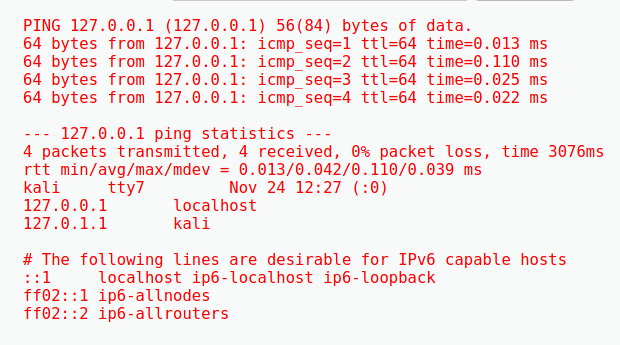
\includegraphics[width=14cm]{img/cmdinjection/output.png}
    \caption{Salida del command injection nivel bajo}
    \label{fig:injOutput}
\end{figure}
Como se aprecia en la figura \ref{fig:injOutput}, el único usuario actual es "kali"
y solo hay 2 nombres de dominio de ipv4 (localhost y kali) y tres nombres de dominio de ipv6
(localhost, ip6-allnodes y ip6-allrouters).
Este ataque no funcionará en otros niveles porque es muy básico.
\paragraph{Nivel medio} Probamos con la entrada del nivel anterior y no funciono, por lo 
que probamos otra forma de ejecutar varios comando en una misma línea. Vimos que hay tres formas
principalmente, con los símbolos ';', '\&\&' y '\textbar \textbar' \cite{multicommand}. 
Tras probar todas las opciones nos dimos cuenta que únicamente estaban verificados lso dos primeros,
por lo que mediante la introducción de los comandos: 
\begin{lstlisting}
a || who
 
\end{lstlisting}
Obtuvimos los valores. En este caso debimos de introducir una ip errónea dado que el operador
'\textbar \textbar' solo ejecuta el segundo comando si falla el primero, por lo que el ping debe fallar.
\begin{figure}[ht!]
    \centering
    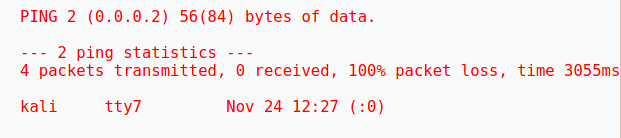
\includegraphics[width=14cm]{img/cmdinjection/medium.png}
    \caption{Salida del command injection nivel medio }
    \label{fig:injOutputMedium}
\end{figure}
Como ejemplo de la salida pondremos la del comando 'who' en la figura \ref{fig:injOutputMedium}, donde se aprecia
que ping ha fallado (100\% packet lost). Esto se deberá a que únicamente han protegido las dos primeras formas 
de concatenar comandos, posiblemente sustituyando esa secuenca de caracteres por espacios. Esto no funcionará 
en niveles más altos si añaden esta tercera secuencia.
\paragraph{Nivel alto} En este ejercicio probamos los mismos comandos que en el nivel medio
y funcionaron aunque con una salida ligeramente distinta.

\begin{figure}[ht!]
    \centering
    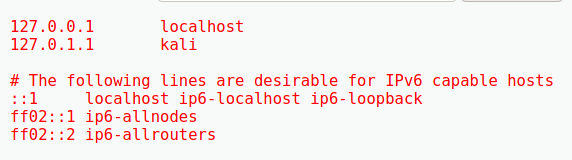
\includegraphics[width=14cm]{img/cmdinjection/hard.png}
    \caption{Salida del command injection nivel alto}
    \label{fig:injOutputHard}
\end{figure}
Como se ve en la figura \ref{fig:injOutputHard} en este caso ya no muestra el ping fallido sino únicamente el 
segundo comando, en este caso el 'cat /etc/hosts'.